\documentclass[11pt,a4paper]{article}
\usepackage[T1]{fontenc}
\usepackage[utf8]{inputenc}
\usepackage[dvipsnames]{xcolor}
\usepackage{mathtools,amsthm}
\usepackage{newpxtext,newpxmath}
\usepackage[a4paper,margin=23mm,headheight=15pt,headsep=8mm,footskip=11mm]{geometry}
\usepackage{microtype,booktabs,array}
\usepackage{tikz}
\usetikzlibrary{arrows.meta,calc,angles,quotes}
\usepackage[most]{tcolorbox}
\usepackage{caption,fancyhdr,enumitem,hyperref}
\hypersetup{colorlinks=true,linkcolor=MidnightBlue,citecolor=MidnightBlue,urlcolor=MidnightBlue,
  pdftitle={A counterexample to the stated pseudo-vertex construction for intersecting convex polygon tours},
  pdfauthor={TouringPolygons project},pdfsubject={Exact geometric counterexample to the local construction in Tan and Jiang, Section 4}}
\definecolor{ink}{HTML}{172C3D}
\definecolor{pOne}{HTML}{3677AD}
\definecolor{pTwo}{HTML}{C78A24}
\definecolor{good}{HTML}{007E72}
\definecolor{bad}{HTML}{B53E62}
\definecolor{quiet}{HTML}{5F707C}
\color{ink}
\setlength{\parindent}{0pt}
\setlength{\parskip}{6pt}
\setlength{\emergencystretch}{1.5em}
\setlist{nosep,leftmargin=1.5em,topsep=4pt}
\captionsetup{font=small,labelfont=bf,skip=6pt}
\pagestyle{fancy}
\fancyhf{}
\fancyhead[L]{\small\sffamily INTERSECTING CONVEX POLYGON TOURS}
\fancyhead[R]{\small\sffamily Technical report}
\fancyfoot[L]{\small\color{quiet}TouringPolygons \enspace / \enspace 13 September 2026}
\fancyfoot[R]{\small\thepage}
\renewcommand{\headrulewidth}{0.35pt}
\newcommand{\norm}[1]{\left\lVert#1\right\rVert}
\newcommand{\dotp}[2]{#1\mathbin{\cdot}#2}
\newcommand{\R}{\mathbb{R}}
\newcommand{\inter}{\operatorname{int}}
\newcommand{\conv}{\operatorname{conv}}
\newcommand{\opt}{\operatorname{OPT}}
\newcommand{\sect}[2]{\section{#1}\label{#2}}
\newtheorem{proposition}{Proposition}
\newtheorem{lemma}{Lemma}
\newtcolorbox{resultbox}[1][]{enhanced,colback=good!5,colframe=good!65!black,
  boxrule=0.6pt,arc=1mm,left=3mm,right=3mm,top=2mm,bottom=2mm,#1}
\tikzset{>=Latex,axis/.style={draw=quiet!50,line width=0.4pt,->},
  one/.style={draw=pOne,fill=pOne!8,line width=0.9pt},
  two/.style={draw=pTwo,fill=pTwo!11,line width=0.9pt},
  route/.style={draw=good,line width=1.5pt},
  wrong/.style={draw=bad,line width=1pt,dashed},
  pt/.style={circle,fill=ink,inner sep=1.6pt},
  lab/.style={font=\small,fill=white,fill opacity=0.88,text opacity=1,inner sep=1.5pt}}

\begin{document}
\thispagestyle{fancy}
{\sffamily\small\color{good}MATHEMATICAL AUDIT \quad / \quad EXACT COUNTEREXAMPLE}\par
\vspace{3mm}
{\LARGE\bfseries A counterexample to the stated\par
pseudo-vertex construction for\par
intersecting convex polygon tours\par}
\vspace{2mm}
{\large Tan and Jiang (TAMC 2017), Section 4}\par
\vspace{2mm}

\begin{resultbox}
\textbf{Main finding.} At a proper intersection of two convex polygon edges,
the unique shortest path to the intersection does not contain enough directional
information to determine the adjacent shortest-path regions. The two
single-reflection rays specified in the published local recipe put two query
targets in the same angular sector, although exactly one target has an optimal
tour bending at that intersection.
\end{resultbox}

This report gives a rational-coordinate instance, original geometric diagrams,
and exact lower bounds proving both optimal tours. The failure concerns the
\emph{stated local construction} in Section 4 of Tan and Jiang~\cite{tan}; it
does not establish that their asymptotic bounds are unattainable, refute the
disjoint-polygon construction, or rule out a corrected algorithm.

\begin{figure}[h!]
\centering
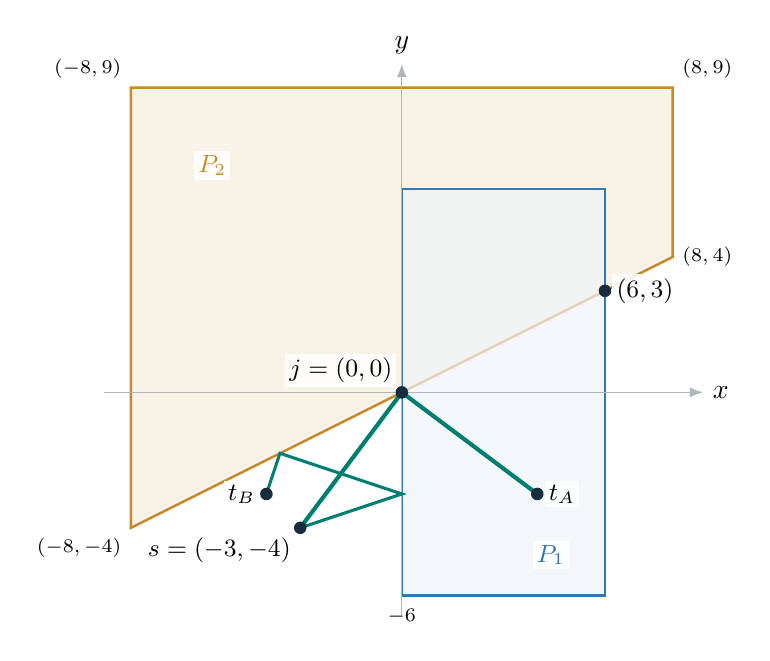
\begin{tikzpicture}[scale=0.43]
  \draw[two] (-8,-4)--(8,4)--(8,9)--(-8,9)--cycle;
  \draw[one,fill opacity=0.7] (0,-6) rectangle (6,6);
  \draw[axis] (-8.8,0)--(8.9,0) node[right] {$x$};
  \draw[axis] (0,-6.6)--(0,9.7) node[above] {$y$};
  \node[lab,text=pTwo] at (-5.6,6.7) {$P_2$};
  \node[lab,text=pOne] at (4.4,-4.8) {$P_1$};
  \draw[route] (-3,-4)--(0,0)--(4,-3);
  \draw[route,line width=1.1pt] (-3,-4)--(0,-3)--(-3.6,-1.8)--(-4,-3);
  \node[pt,label={[lab]below left:$s=(-3,-4)$}] at (-3,-4) {};
  \node[pt,label={[lab]above left:$j=(0,0)$}] at (0,0) {};
  \node[pt,label={[lab]right:$(6,3)$}] at (6,3) {};
  \node[pt,label={[lab]right:$t_A$}] at (4,-3) {};
  \node[pt,label={[lab]left:$t_B$}] at (-4,-3) {};
  \node[font=\scriptsize,anchor=north] at (0,-6.1) {$-6$};
  \node[font=\scriptsize,anchor=south east] at (-8,9) {$(-8,9)$};
  \node[font=\scriptsize,anchor=south west] at (8,9) {$(8,9)$};
  \node[font=\scriptsize,anchor=north east] at (-8,-4) {$(-8,-4)$};
  \node[font=\scriptsize,anchor=west] at (8,4) {$(8,4)$};
\end{tikzpicture}
\caption{The complete instance, drawn at equal scale on both axes. Blue is the
first polygon, amber the second. Green shows the two optimal tours, proved
independently in Sections~\ref{sec:a} and~\ref{sec:b}. Only the tour to $t_A$
visits both polygons at $j$.}
\label{fig:overview}
\end{figure}

\textbf{Reading guide.} Sections 1--3 state the model and the contradiction;
Sections 4--5 prove global optimality and uniqueness; Sections 6--7 identify
the lost information; Sections 8--9 delimit the conclusion and give reproduction
details. All geometric figures in this report are original vector drawings.

\clearpage
\sect{Problem and published construction}{sec:model}

\textbf{Ordered visits.} A tour is a rectifiable curve from $s$ to $t$ with
nondecreasing parameters $\tau_1\leq\tau_2$ such that its point at $\tau_i$
belongs to the closed polygon $P_i$. Equality is permitted: one point may satisfy
two consecutive visits. The polygons are regions to visit, not obstacles.
Traversing or revisiting their interiors is allowed.

Choosing ordered contacts $a\in P_1$, $b\in P_2$ and straightening the three
subcurves cannot increase length. Conversely, the polygonal chain through any
such $a,b$ is a feasible ordered tour. Consequently,
\begin{equation}
  \opt(t)=\min_{a\in P_1,\ b\in P_2}
  F_t(a,b),\qquad
  F_t(a,b)=\norm{a-s}+\norm{b-a}+\norm{t-b}.
  \label{eq:objective}
\end{equation}
This reduction means the lower bounds below apply to every feasible curve,
not merely to a selected list of candidate paths.

\textbf{The map being constructed.} A last-step shortest-path map classifies
query points according to how an optimal prefix tour interacts with the current
polygon: reflection at an edge, bending at a vertex, or crossing. A correct
bending cell at $j$ must support extending the shortest prefix to $j$ directly
to the query point. Its boundaries must separate this behavior from the
neighboring contact patterns.

For intersecting polygons, Tan and Jiang split original boundary edges at their
intersections with earlier polygon boundaries, creating \emph{pseudo-vertices}
and \emph{pseudo-edges}~\cite[Section 4, pp.~620--621]{tan}. At a pseudo-vertex
$j\in\partial P_{i+1}\cap\partial P_h$, their paragraph immediately below
Figure 4 states the following local recipe:
\begin{enumerate}
  \item A bending region can exist only if $j$ lies inside all intermediate
  polygons $P_{h+1},\ldots,P_i$ and the shortest prefix to $j$ enters neither
  $\inter P_h$ nor $\inter P_{i+1}$.
  \item Its bounding rays are obtained by reflecting the last segment of that
  shortest prefix on the incident edges of $P_h$ and $P_{i+1}$, respectively.
  \item One adjacent region is a crossing region; the other is a reflection
  region.
\end{enumerate}
The counterexample targets the literal two-single-reflection rule in item 2,
and also contradicts the adjacency description in item 3. The first item is
only a necessary condition; the proof below independently establishes that a
bending region actually exists.

\begin{resultbox}[colback=pOne!5,colframe=pOne!70!black]
\textbf{The distinction to track.} The last nonzero segment of the path
\emph{at} $j$ and the limiting last-segment direction of paths to points
\emph{approaching} $j$ are different data. Uniqueness of the path at $j$ does
not make those one-sided limits equal.
\end{resultbox}

\textbf{Source interpretation.} The original published PDF, including its
Figure 4 and accompanying paragraph, was checked against the local TeX
transcription. This is not a transcription error. If the wording is intended
to require additional unfolding or one-sided limiting information, that
additional operation must be specified and justified; the calculation using
the two individual reflections of the single incoming segment fails as shown
here.

\clearpage
\sect{An exact instance satisfying the stated assumptions}{sec:instance}

Take the source, ordered polygons, and query targets to be
\begin{align}
 s&=(-3,-4), & j&=(0,0),\notag\\
 P_1&=[0,6]\times[-6,6],\notag\\
 P_2&=\conv\{(-8,-4),(8,4),(8,9),(-8,9)\}\notag\\
    &=\{(x,y):-8\leq x\leq8,\ x/2\leq y\leq9\},\notag\\
 t_A&=(4,-3), & t_B&=(-4,-3).
 \label{eq:instance}
\end{align}
The vertices displayed for $P_2$, and the order
$(0,-6),(6,-6),(6,6),(0,6)$ for $P_1$, are counterclockwise.

Both polygons are bounded and convex, with positive area. Their boundaries
cross properly at $j=(0,0)$ and $(6,3)$, strictly inside the corresponding
edges. There are no shared edges and no point at which three edges intersect.
The relevant supporting lines at $j$ are
\begin{equation}
 \ell_1:\ x=0,\qquad \ell_2:\ y=x/2.
 \label{eq:lines}
\end{equation}
They are neither parallel nor perpendicular. The source is outside $P_1$;
both query targets are outside $P_2$. The fact that $t_A$ is in $P_1$ is
permitted by the ordered-tour problem.

The unique shortest prefix to $j$ is the segment $s\to j$, of length $5$.
It first reaches each polygon at $j$, entering neither interior. With only two
polygons, there are no intermediate polygons, so the first condition in the
published recipe is vacuous and the second is satisfied. The unit incoming
direction is
\begin{equation}
 u=\frac{j-s}{\norm{j-s}}=\left(\frac35,\frac45\right).
\end{equation}
Reflection of a direction vector in $\ell_1$ or $\ell_2$ is given by
\begin{equation}
 R_1=\begin{pmatrix}-1&0\\0&1\end{pmatrix},\qquad
 R_2=\begin{pmatrix}3/5&4/5\\4/5&-3/5\end{pmatrix}.
 \label{eq:reflections}
\end{equation}
Thus the two specified single-reflection directions are
\begin{equation}
 \boxed{R_1u=(-3/5,4/5)},\qquad \boxed{R_2u=(1,0)}.
 \label{eq:paper-rays}
\end{equation}

\begin{center}
\renewcommand{\arraystretch}{1.22}
\begin{tabular}{@{}lll@{}}
\toprule
Query & Unique optimal contacts $(a,b)$ & Optimal length\\
\midrule
$t_A=(4,-3)$ & $(j,j)$ & $10$\\
$t_B=(-4,-3)$ & $((0,-3),(-18/5,-9/5))$ & $13\sqrt{10}/5\approx8.2219219164$\\
\bottomrule
\end{tabular}
\end{center}
The table is certified in Sections~\ref{sec:a} and~\ref{sec:b}. In particular,
it is independent of the repository's production solver and of any numerical
optimization routine.

\clearpage
\sect{Why the specified rays cannot define the bending region}{sec:contradiction}

Angles here are measured counterclockwise from the positive $x$-axis. The two
specified rays have angles $126.8699^\circ$ and $0^\circ$. Both target directions
lie strictly inside their major angular sector:
\[
 \arg(t_B)=216.8699^\circ,\qquad \arg(t_A)=323.1301^\circ.
\]
Yet the optimal tour to $t_A$ bends at $j$, and the unique optimal tour to $t_B$
does not. Both targets are below $\ell_2$, so excluding the current polygon's
interior cannot resolve this discrepancy.

\begin{figure}[h!]
\centering
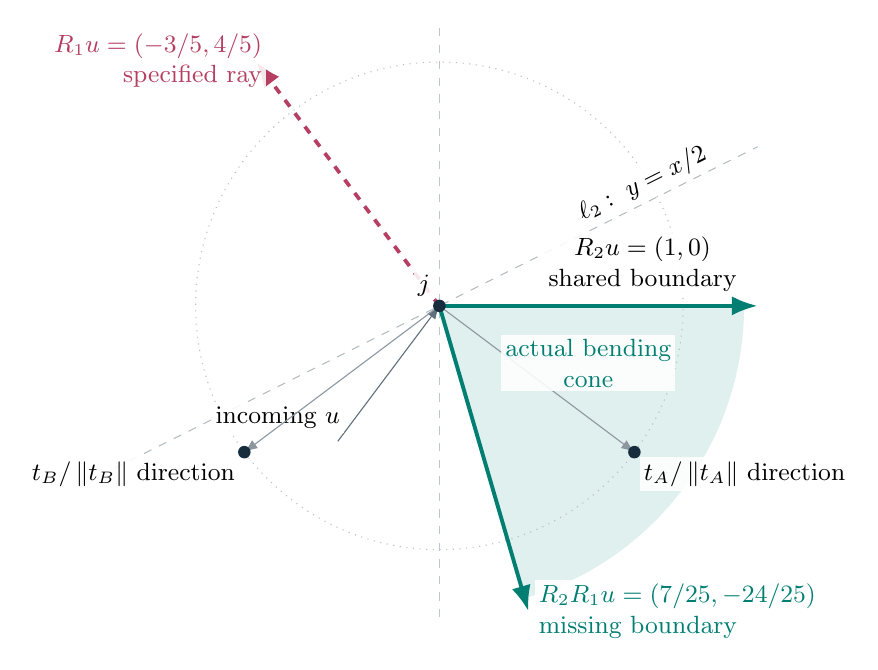
\begin{tikzpicture}[scale=0.86]
  \fill[good!12] (0,0)--(4.5,0) arc[start angle=0,end angle=-73.7397953,radius=4.5]--cycle;
  \draw[quiet!45,dotted] (0,0) circle (3.6);
  \draw[quiet!45,dashed] (-4.8,-2.4)--(4.7,2.35);
  \node[lab,rotate=26.565] at (3,1.8) {$\ell_2:\ y=x/2$};
  \draw[quiet!40,dashed] (0,-4.6)--(0,4.1);
  \draw[bad,dashed,line width=1.35pt,->] (0,0)--(-2.7,3.6);
  \node[lab,text=bad,anchor=east,align=right] at (-2.55,3.62)
    {$R_1u=(-3/5,4/5)$\\specified ray};
  \draw[good,line width=1.4pt,->] (0,0)--(4.7,0);
  \node[lab,anchor=south,align=center] at (3.0,0.15)
    {$R_2u=(1,0)$\\shared boundary};
  \draw[good,line width=1.4pt,->] (0,0)--(1.316,-4.512);
  \node[lab,anchor=north west,align=left,text=good] at (1.4,-4.04)
    {$R_2R_1u=(7/25,-24/25)$\\missing boundary};
  \draw[quiet,->] (-1.5,-2)--(0,0);
  \node[lab,anchor=east] at (-1.4,-1.65) {incoming $u$};
  \draw[ink!50,->] (0,0)--(2.88,-2.16);
  \draw[ink!50,->] (0,0)--(-2.88,-2.16);
  \node[pt,label={[lab]below right:$t_A/\norm{t_A}$ direction}] at (2.88,-2.16) {};
  \node[pt,label={[lab]below left:$t_B/\norm{t_B}$ direction}] at (-2.88,-2.16) {};
  \node[lab,text=good,align=center] at (2.2,-0.85) {actual bending\\cone};
  \node[pt,label={[lab]above left:$j$}] at (0,0) {};
\end{tikzpicture}
\caption{Direction diagram centered at $j$; marked target directions are placed
at a common radius. The two specified rays fail to separate $t_A$ from $t_B$.
The green sector uses the correct lower boundary, derived from one-sided
limits in Section~\ref{sec:limits}. It contains $t_A$ and excludes $t_B$.}
\label{fig:rays}
\end{figure}

\begin{proposition}
Neither angular sector bounded by the two rays in
\eqref{eq:paper-rays} is the bending region of $j$ for this instance.
\end{proposition}
\begin{proof}
The smaller sector excludes $t_A$, whose unique optimum bends at $j$. The
larger sector contains $t_B$, whose unique optimum does not bend at $j$.
The optimality and uniqueness assertions are proved next. The targets are
strictly away from the ray boundaries, so no boundary tie convention changes
the contradiction.
\end{proof}

\clearpage
\sect{A global certificate for the tour that bends at the intersection}{sec:a}

\begin{lemma}[Supporting-vector lower bound]
For any vectors $d_0,d_1,d_2$ with $\norm{d_i}\leq1$ and any contacts $a,b$,
\begin{align}
 F_t(a,b)\ &\geq -\dotp{d_0}{s}+\dotp{d_2}{t}
  +\dotp{(d_0-d_1)}{a}+\dotp{(d_1-d_2)}{b}.
 \label{eq:certificate}
\end{align}
\end{lemma}
\begin{proof}
Apply $\norm{v}\geq\dotp{d}{v}$ separately to $a-s$, $b-a$, and $t-b$, then
collect terms. If $\norm{d}<1$, equality in this inequality forces $v=0$.
If $\norm{d}=1$, equality forces $v$ to be a nonnegative multiple of $d$.
\end{proof}

For $t_A=(4,-3)$, the proposed contacts are $a=b=j$. They yield
\[
 F_{t_A}(j,j)=\norm{(3,4)}+0+\norm{(4,-3)}=5+5=10.
\]
Set
\begin{equation}
 d_0=u=\left(\frac35,\frac45\right),\qquad
 d_1=z=\left(\frac1{10},\frac45\right),\qquad
 d_2=w_A=\left(\frac45,-\frac35\right).
\end{equation}
Both $u$ and $w_A$ are unit vectors, while $\norm{z}^2=13/20<1$. Their
differences align with inward normals of the two active supporting lines:
\[
 u-z=(1/2,0),\qquad z-w_A=(-7/10,7/5).
\]
Substituting in Lemma 1 gives, for \emph{every} feasible pair of contacts,
\begin{align}
 F_{t_A}(a,b)
 &\geq 10+\frac12a_x+\frac75\left(b_y-\frac12b_x\right)\notag\\
 &\geq10.
 \label{eq:a-proof}
\end{align}
The final inequality follows solely from $a_x\geq0$ in $P_1$ and
$b_y-b_x/2\geq0$ in $P_2$. No assumption has been made that the optimum
touches these particular edges; the bound covers the entire polygons.

\begin{proposition}
The unique optimal geometric tour to $t_A$ is $s\to j\to t_A$, of length $10$.
\end{proposition}
\begin{proof}
The displayed tour attains the lower bound. To attain equality in
\eqref{eq:a-proof}, both supporting terms must vanish, giving $a_x=0$ and
$b_y=b_x/2$. Since $\norm{z}<1$, equality in the middle norm bound also forces
$a=b$. The two supporting lines intersect only at $j$, so $a=b=j$.
The remaining curve portions must be straight to attain equality in the
straightening argument. Uniqueness is geometric; pauses or reparametrizations
do not count as different tours.
\end{proof}

\begin{resultbox}
\textbf{This is a true cell, not an isolated coincidence.} The multipliers
$1/2$ and $7/5$ are strictly positive, and $\norm{z}<1$. These inequalities
persist for sufficiently small changes of the target direction. Section~\ref{sec:cone}
computes the full bending cone on the exterior side of the active edge.
\end{resultbox}

\clearpage
\sect{A shorter, uniquely optimal tour in the same specified sector}{sec:b}

For $t_B=(-4,-3)$, take
\begin{equation}
 a^*=(0,-3),\qquad b^*=\left(-\frac{18}{5},-\frac95\right).
 \label{eq:b-contacts}
\end{equation}
These points are in the relative interiors of $P_1$'s left edge and $P_2$'s
lower edge, respectively. The three segment vectors are
$(3,1)$, $(6/5)(-3,1)$, and $(2/5)(-1,-3)$, so the path length is
\begin{equation}
 \norm{a^*-s}+\norm{b^*-a^*}+\norm{t_B-b^*}
   =\left(1+\frac65+\frac25\right)\sqrt{10}=\frac{13}{5}\sqrt{10}.
 \label{eq:b-length}
\end{equation}

\begin{figure}[h!]
\centering
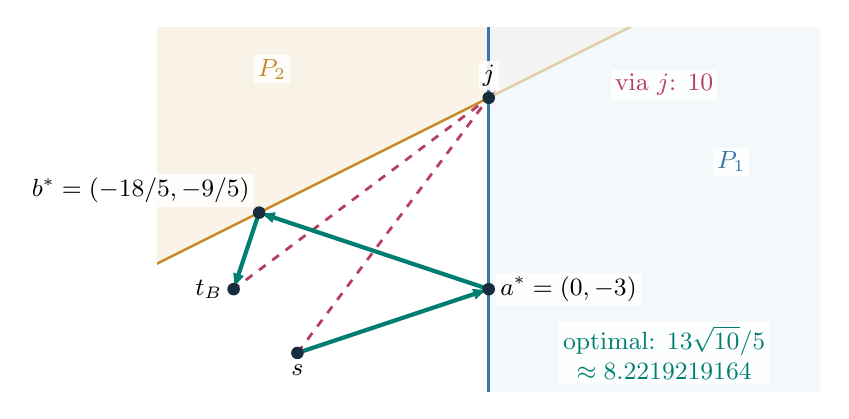
\begin{tikzpicture}[scale=0.81]
  \begin{scope}
    \clip (-5.2,-4.6) rectangle (5.2,1.1);
    \draw[two] (-8,-4)--(8,4)--(8,9)--(-8,9)--cycle;
    \draw[one,fill opacity=0.65] (0,-6) rectangle (6,6);
    \draw[wrong] (-3,-4)--(0,0)--(-4,-3);
    \draw[route,-{Latex[length=2mm]}] (-3,-4)--(0,-3);
    \draw[route,-{Latex[length=2mm]}] (0,-3)--(-3.6,-1.8);
    \draw[route,-{Latex[length=2mm]}] (-3.6,-1.8)--(-4,-3);
  \end{scope}
  \node[pt,label={[lab]below:$s$}] at (-3,-4) {};
  \node[pt,label={[lab]above:$j$}] at (0,0) {};
  \node[pt,label={[lab]right:$a^*=(0,-3)$}] at (0,-3) {};
  \node[pt,label={[lab]above left:$b^*=(-18/5,-9/5)$}] at (-3.6,-1.8) {};
  \node[pt,label={[lab]left:$t_B$}] at (-4,-3) {};
  \node[lab,text=pOne] at (3.8,-1) {$P_1$};
  \node[lab,text=pTwo] at (-3.4,0.45) {$P_2$};
  \node[lab,text=bad,align=center] at (2.75,0.2) {via $j$: $10$};
  \node[lab,text=good,align=center] at (2.75,-4)
    {optimal: $13\sqrt{10}/5$\\$\approx 8.2219219164$};
\end{tikzpicture}
\caption{Close view of the tour to $t_B$ with polygon interiors cropped to the
viewport. The green route reflects first on $P_1$, then on $P_2$. The dashed
route through $j$ is feasible but strictly longer. Axes use the same scale.}
\label{fig:b}
\end{figure}

Let $U=(3,1)/\sqrt{10}$, $Z=(-3,1)/\sqrt{10}$, and
$W=(-1,-3)/\sqrt{10}$. They are the three unit segment directions, and
$R_1U=Z$, $R_2Z=W$. Lemma 1 yields
\begin{equation}
 F_{t_B}(a,b)\geq\frac{13}{5}\sqrt{10}
  +\frac6{\sqrt{10}}a_x
  +\frac4{\sqrt{10}}\left(b_y-\frac12b_x\right)
  \geq\frac{13}{5}\sqrt{10}.
 \label{eq:b-proof}
\end{equation}
Equality is attained at \eqref{eq:b-contacts}, proving global optimality.
For equality, the positive supporting multipliers force $a_x=0$ and $b_y=b_x/2$.
The first norm equality forces $a-s$ to have direction $U$, fixing
$a=a^*$. The second forces $b-a^*$ to have direction $Z$, fixing $b=b^*$.
The straightening argument again establishes uniqueness of the geometric tour.

Any tour going through $j$ has length at least
$\norm{j-s}+\norm{t_B-j}=10$. The incorrect bend-at-$j$ choice therefore loses
exactly
\[
 \boxed{10-\frac{13}{5}\sqrt{10}\approx1.7780780836}.
\]

\clearpage
\sect{The missing information: two different one-sided limits}{sec:limits}

Let $\pi_1(q)$ denote a shortest path from $s$ visiting $P_1$ and ending at $q$.
Approach $j$ on the lower edge of $P_2$ using
\[
 q_+(\varepsilon)=(2\varepsilon,\varepsilon),\qquad
 q_-(\varepsilon)=(-2\varepsilon,-\varepsilon),\qquad \varepsilon>0.
\]
For all sufficiently small $\varepsilon$, $q_+$ lies in $P_1$, so
$\pi_1(q_+)$ is the straight segment from $s$ and its last direction tends to
$u=(3/5,4/5)$.

In contrast, $q_-$ lies outside $P_1$. Unfolding in $x=0$ gives a unique
reflection contact
\begin{equation}
 a_\varepsilon=\left(0,-\frac{11\varepsilon}{3+2\varepsilon}\right),\qquad
 \pi_1(q_-):s\longrightarrow a_\varepsilon\longrightarrow q_-.
 \label{eq:epsilon-contact}
\end{equation}
Indeed, the segment from $s$ to the reflected endpoint $(2\varepsilon,-\varepsilon)$
meets $x=0$ at this point; the contact is inside the finite edge. Minimizing
over the half-plane $x\geq0$ provides the same reflection lower bound, so this
is also optimal for the rectangle. Its final unit direction satisfies
\begin{equation}
 \lim_{\varepsilon\downarrow0}
 \frac{q_-(\varepsilon)-a_\varepsilon}
      {\norm{q_-(\varepsilon)-a_\varepsilon}}
   =\left(-\frac35,\frac45\right)=R_1u.
 \label{eq:one-sided}
\end{equation}

\begin{figure}[h!]
\centering
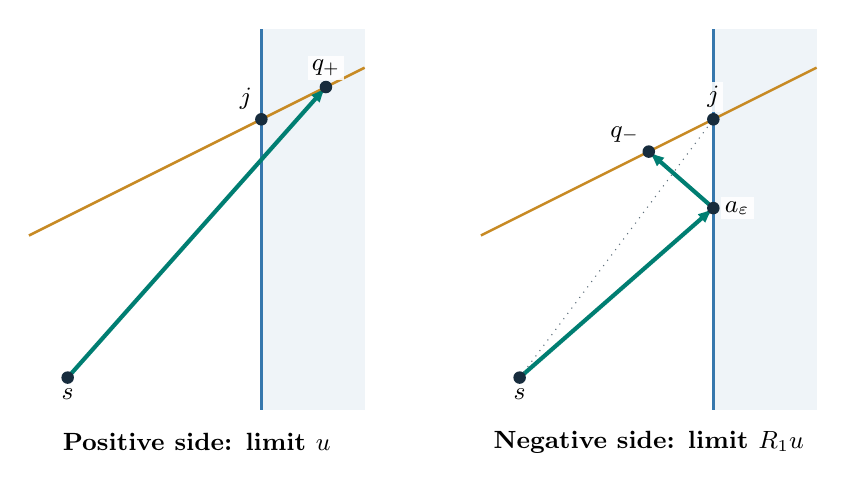
\begin{tikzpicture}[scale=0.82]
  \begin{scope}
    \fill[pOne!8] (0,-4.5) rectangle (1.6,1.4);
    \draw[pOne,line width=0.9pt] (0,-4.5)--(0,1.4);
    \draw[pTwo,line width=0.9pt] (-3.6,-1.8)--(1.6,0.8);
    \draw[route,-{Latex[length=2mm]}] (-3,-4)--(1,0.5);
    \node[pt,label={[lab]below:$s$}] at (-3,-4) {};
    \node[pt,label={[lab]above left:$j$}] at (0,0) {};
    \node[pt,label={[lab]above:$q_+$}] at (1,0.5) {};
    \node[font=\small\bfseries] at (-1,-5) {Positive side: limit $u$};
  \end{scope}
  \begin{scope}[xshift=7cm]
    \fill[pOne!8] (0,-4.5) rectangle (1.6,1.4);
    \draw[pOne,line width=0.9pt] (0,-4.5)--(0,1.4);
    \draw[pTwo,line width=0.9pt] (-3.6,-1.8)--(1.6,0.8);
    \draw[route,-{Latex[length=2mm]}] (-3,-4)--(0,-1.375);
    \draw[route,-{Latex[length=2mm]}] (0,-1.375)--(-1,-0.5);
    \draw[quiet,dotted] (-3,-4)--(0,0);
    \node[pt,label={[lab]below:$s$}] at (-3,-4) {};
    \node[pt,label={[lab]above:$j$}] at (0,0) {};
    \node[pt,label={[lab]above left:$q_-$}] at (-1,-0.5) {};
    \node[pt,label={[lab]right:$a_\varepsilon$}] at (0,-1.375) {};
    \node[font=\small\bfseries] at (-1,-5) {Negative side: limit $R_1u$};
  \end{scope}
\end{tikzpicture}
\caption{Two approaches to $j$, drawn with $\varepsilon=1/2$ so the shrinking
segment is visible. Blue shading denotes $P_1$ locally; amber is the supporting
edge of $P_2$. Both complete paths converge to $s\to j$, but their last-segment
directions have different limits.}
\label{fig:limits}
\end{figure}

The final segment on the negative side shrinks to zero length as
$\varepsilon\downarrow0$. It is absent from the unique path \emph{at} $j$.
Reflecting the two incoming limits in the \emph{current} edge $\ell_2$ gives
\begin{equation}
 r_+=R_2u=(1,0),\qquad
 \boxed{r_-=R_2R_1u=(7/25,-24/25)}.
 \label{eq:true-rays}
\end{equation}
The composition is essential: $R_2R_1u\neq R_1u$. On both sides the prefix
approaches the lower edge from outside $P_2$; the two adjacent current-polygon
cells are reflection regions. A bending cone lies between their limiting rays.

\clearpage
\sect{An exact description of the exterior-side bending cone}{sec:cone}

The limiting-ray calculation can also be checked directly by convex optimality.
Let $q\neq j$ be below the active line, $q_y<q_x/2$, and put
$w=q/\norm{q}$. At $a=b=j$, the first and last norm terms have gradients $u$
and $w$, while the subgradient of the zero middle segment is the closed unit
disk. The normal-cone condition for minimizing the convex objective
\eqref{eq:objective} over $P_1\times P_2$ is therefore
\begin{equation}
 \begin{split}
 u-z&=\lambda(1,0),\\
 z-w&=\mu(-1/2,1),
 \end{split}
 \qquad \norm{z}\leq1,\quad \lambda,\mu\geq0.
 \label{eq:kkt}
\end{equation}
These conditions are necessary and sufficient: the objective is finite,
continuous, and convex, and the only active polygon constraints at $j$ are the
two supporting lines. Equivalently, sufficiency follows immediately from
Lemma 1, with equality at $j$.

Writing $c=w_x+w_y/2$, equations~\eqref{eq:kkt} imply
\begin{equation}
 z_y=\frac45,\qquad z_x=c-\frac25,\qquad
 \lambda=1-c,\qquad\mu=\frac45-w_y.
\end{equation}
Thus feasibility is exactly
\begin{equation}
 -\frac15\leq w_x+\frac12w_y\leq1,\qquad w_y\leq\frac45.
 \label{eq:unit-conditions}
\end{equation}
Intersecting these inequalities with the unit circle and the exterior-side
condition $w_y<w_x/2$ leaves the closed arc from
$(7/25,-24/25)$ to $(1,0)$. Hence the set of these queries for which contacts
$a=b=j$ are optimal is precisely
\begin{equation}
 \boxed{\mathcal C_j=\{(x,y)\neq(0,0):y\leq0,\ 24x+7y\geq0\}}.
 \label{eq:cone}
\end{equation}
Its angular width is approximately $73.7398^\circ$. In its angular interior,
the support multipliers are positive and $\norm{z}<1$, which forces the two
contacts to equal $j$ exactly as in Section~\ref{sec:a}.

For the two witnesses,
\[
 24(t_A)_x+7(t_A)_y=75>0,\qquad
 24(t_B)_x+7(t_B)_y=-117<0.
\]
This is an exact algebraic separation, with substantial margins. The
contradiction is not caused by floating-point roundoff, a target on a cell
boundary, perpendicular edges, or nonunique optimal tours.

\textbf{Why restrict to the exterior side?} The map treats the interior of
$P_2$ as crossing. If the unit-circle calculation is performed without the
condition $w_y<w_x/2$, it also retains the isolated directions $u$ and $R_1u$,
which enter $P_2$ near $j$. They do not enlarge the two-dimensional exterior
bending cell. Equation~\eqref{eq:cone} describes precisely the side relevant
to both targets and Figure~\ref{fig:rays}; it does not silently equate interior
crossing behavior with exterior bending behavior.

\clearpage
\sect{What fails, and what a correction would need}{sec:scope}

\textbf{The failed inference.} Splitting edges at intersections is necessary,
but the coordinates of a pseudo-vertex and the unique prefix path to it do not
determine both incident directional limits. Here the negative-side limit
remembers an earlier reflection even though its final segment vanishes at $j$.
Replacing that limit by the last segment of the endpoint path loses one
reflection and rotates a true boundary to the wrong direction.

The resulting issue is structural. A circular locator, whether scanned
linearly or searched by binary search, cannot repair incorrectly defined
regions. The two query witnesses must receive different bending classifications,
and the stated pair of bounding rays cannot supply that distinction. For the
major-sector interpretation, extending the prefix through $j$ to $t_B$ returns
a feasible path with a strictly incorrect length. For the minor-sector
interpretation, the true bending optimum for $t_A$ is omitted.

\textbf{Relation to Dror et al.} The earlier starburst construction explicitly
defines vertex behavior using limits of outgoing rays as their source
approaches the vertex along incident first-contact-tree edges~\cite[Section
4.1, Claim 1 immediately before Lemma 7, p.~477]{dror}. Those limits retain
exactly the information distinguished in Figure~\ref{fig:limits}. This
counterexample is compatible with that formulation. It does not prove that
Dror's entire construction can be substituted into the present implementation
without further work, nor that all of its details have been audited here.

\textbf{Requirements for a corrected construction.}
\begin{enumerate}
 \item Represent or compute the incident one-sided prefix directions at a
 pseudo-vertex, including directions carried by segments that vanish at the
 endpoint. A query keyed only by point and visit index may require an
 additional incident-side state.
 \item Reflect those limits in the current supporting edge and account for
 the resulting vertex fan. Distinguish reflection on an earlier polygon from
 reflection on the current polygon.
 \item Prove that the complete inherited crossing, reflection, and bending
 regions cover the query domain and have the boundary order required by the
 locator. Closed contacts and coincident consecutive visits must preserve the
 prescribed visit order.
 \item Re-establish construction, storage, and reporting bounds for this
 richer representation. Degeneracies outside the paper's no-three-edges
 assumption need their own treatment if an implementation accepts them.
\end{enumerate}

\begin{resultbox}
\textbf{Scope of the conclusion.} The example refutes the stated local
two-single-reflection recipe and the crossing/reflection adjacency assertion.
Consequently that recipe does not justify a generally correct intersecting
solver. It does \emph{not} prove the nonexistence of a corrected polynomial
algorithm or invalidate the claimed complexity bounds as existential bounds.
Theorem 2's construction requires additional justification or repair; the
present report does not supply a complete replacement algorithm.
\end{resultbox}

The repository also contains implementation failures, including a
common-intersection shortcut that returns $10$ on the second witness. That
code is not a faithful implementation of the published local construction,
so its output is not used as evidence against the paper. The mathematical
contradiction rests entirely on the independently proved tours above.

\clearpage
\sect{Reproduction and source locations}{sec:reproduce}
\setlength{\parskip}{4pt}

All coordinates, optimal contacts, reflection matrices, and supporting vectors
are explicit. The proof uses Euclidean norm inequalities and polygon support
constraints, without numerical tolerances or an optimizer. Decimal lengths and
angles illustrate the figures; they are not premises of the proof.

\textbf{Repository artifacts.} Paths below are relative to the repository root.
The existing audit program constructs both witnesses directly and checks their
primal and supporting-vector certificates.
\begin{center}
\small
\renewcommand{\arraystretch}{1.25}
\begin{tabular}{@{}p{0.24\textwidth}p{0.71\textwidth}@{}}
\toprule
Artifact & Location\\
\midrule
This LaTeX source & \path{docs/reports/intersection-counterexample/report.tex}\\
Full audit & \path{docs/algorithms/intersecting-tpp-audit.md}\\
Certificate harness & \path{packages/convex-tpp/cpp/src/main-intersection_audit.cpp}\\
Harness instructions & \path{benchmarks/suites/intersection-audit/README.md}\\
\bottomrule
\end{tabular}
\end{center}

To rebuild the report with a TeX distribution providing \texttt{latexmk},
\texttt{pdflatex}, TikZ, and the New PX fonts:
\begin{quote}\small
\verb|bash docs/reports/intersection-counterexample/build.sh|
\end{quote}
The output is \path{output/pdf/intersection-counterexample.pdf}.
The proof-only harness, built according to the fixture README, was rerun for
this report:
\begin{quote}\small
\verb|.build/intersection-audit/tpp-convex --proof-only|\par
\verb|Checks=99, failures=0 (proof_only=1)|
\end{quote}
This checks the proof fixtures and auxiliary audit invariants; it is not a
claim that the production solver passes the full intersection audit. No
production solver was changed while preparing this report.

\textbf{Original-source locators.} Printed page numbers and PDF positions
(counted from 1) are listed below. The statements were checked in the original PDFs.
\begin{center}
\small
\renewcommand{\arraystretch}{1.18}
\begin{tabular}{@{}p{0.16\textwidth}p{0.21\textwidth}p{0.57\textwidth}@{}}
\toprule
Source & Location & Relevant content\\
\midrule
Tan--Jiang & pp.~620--621; PDF 7--8 & Boundary splitting; Figure 4 and paragraph below it giving the pseudo-vertex rays and adjacent region types.\\
Tan--Jiang & p.~622; PDF 9 & Theorem 2: $O(k^2n)$ construction, $O(kn)$ storage and path reporting, with $n$ total input vertices.\\
Dror et al. & p.~477; PDF 5 & Section 4.1, Claim 1 before Lemma 7: limiting rays along incident tree edges.\\
\bottomrule
\end{tabular}
\end{center}

\begingroup
\small
\setlength{\parskip}{3pt}
\begin{thebibliography}{2}
\bibitem{tan} Xuehou Tan and Bo Jiang.
\emph{Efficient Algorithms for Touring a Sequence of Convex Polygons and Related
Problems}. TAMC 2017, Lecture Notes in Computer Science 10185, pp.~614--627.
\href{https://doi.org/10.1007/978-3-319-55911-7_44}{doi:10.1007/978-3-319-55911-7\_44}.
Local original: \path{docs/bibliography/TPP-Tan&Jiang/original.pdf}.
\bibitem{dror} Moshe Dror, Alon Efrat, Anna Lubiw, and Joseph S. B. Mitchell.
\emph{Touring a Sequence of Polygons}. Proceedings of STOC 2003, pp.~473--482.
\href{https://doi.org/10.1145/780542.780612}{doi:10.1145/780542.780612}.
Local original: \path{docs/bibliography/TPP-Dror/original.pdf}.
\end{thebibliography}
\endgroup
\end{document}
